% revision history
%
% 20170518 NPS: Initial draft
% 20170721 CC: approved by the Board

\documentclass[11pt]{article}
\usepackage{fancyhdr}
\usepackage{authblk}
\usepackage{graphicx}
\usepackage{url}
\topmargin=-5mm
\evensidemargin=0cm
\oddsidemargin=0cm
\textwidth=16cm
\textheight=22cm
\addtolength{\headheight}{1.6pt}
\newcommand{\cancel}[1]{}
\newcommand{\mymark}{$^*$}

\newcommand{\lastupdate}{Nov. 2024}

\lhead{\sc Provenance Detection for AI-Generated Images}
\rhead{\sc \lastupdate}

\title{\bf Private and Robust AI Image Provenance Detection Using Fuzzy Hashing and MP-FHE}
% \author{Shree Singhi, Aayan Yadav, Aayush Gupta, Shahriar Ebrahimi, Parisa Hassanizadeh}


\author[1,2]{Shree Singhi}
\author[1,2]{Aayan Yadav}
\author[3]{Aayush Gupta}
\author[4]{Shahriar Ebrahimi}
\author[4,5]{Parisa Hassanizadeh}
\affil[1]{Zellic}
\affil[2]{Indian Institute of Technology Roorkee: \{\textit{shree\_s, aayan\_y}\} @\textit{mfs.iitr.ac.in}}
\affil[3]{ZK Email: \textit{aayushg@mit.edu}}
\affil[4]{IDEAS NCBR: \{\textit{shahriar.ebrahimi, parisa.hassanizadeh}\} @\textit{ideas-ncbr.pl}}
% \affil[2]{University of Warsaw, Poland}
\affil[5]{Polish Academy of Science, Poland}
% \affil[ ]{\{\textit{shree\_s, aayan\_y}\} @\textit{mfs.iitr.ac.in}$^2$, \textit{aayushg@mit.edu}$\:^3$, \{\textit{shahriar.ebrahimi, parisa.hassanizadeh}\} @\textit{ideas-ncbr.pl}$^4$}



\date{\lastupdate
 \footnote{The PoC implementation is available at \protect\url{https://github.com/proteus-photos/proteus-aegis}}}

\providecommand{\note}[1]{[[\textsf{#1}]]}
\providecommand{\todo}[1]{\note{TODO: #1}}

\begin{document}
\maketitle

\thispagestyle{empty}
\pagenumbering{roman}

\par\noindent
\textbf{Abstract.} The rapid rise of AI-generated images has created a critical challenge in distinguishing authentic content from fabricated media, posing significant risks to privacy, security, and intellectual property rights. Existing solutions, such as watermarking, fall short in addressing these challenges as they are easily defeated by transformations like filters, compression during social media sharing, and screenshots. Moreover, watermarking is vulnerable to removal or manipulation, particularly when models are open-sourced or leaked. Compounding the issue, creators of digital media face increasing difficulties in protecting their intellectual property, as current provenance systems can inadvertently validate unauthorized or AI-generated content, undermining copyright claims. We develop a state-of-the-art perceptual hashing model, DinoHash, derived from DinoV2, robust to common transformations like filters, compression and crops.  However, to ensure privacy and security in real-world applications, we integrate a Multi-Party Fully Homomorphic Encryption (MP-FHE) scheme into our framework. MP-FHE plays a critical role by allowing secure, privacy-preserving queries and registry operations, ensuring that neither the user data nor the perceptual hashes are exposed at any point during processing.  Furthermore, we improve previous work on AI-generated media detection. This approach is useful in cases where the content is absent from our registry. This comprehensive solution directly addresses the global need for robust content verification and copyright protection, offering a 12\% improvement in bit accuracy over the state-of-the-art watermarking with a consistent edge in true positive rate~(TPR) and false positive rate~(FPR) tradeoffs across a wide range of transformations. Our AI-generated media detection results perform consistently better showing a 25\% improvement in classification accuracy on commonly used real-world AI image generators than existing algorithms. By combining perceptual hashing, MP-FHE, and an AI content detection model, our proposed framework provides better robustness and privacy compared to previous work.

\pagebreak
% \tableofcontents

\pagebreak
\pagestyle{fancy}
\pagenumbering{arabic}


\begin{figure*}[!t]
    \centering
    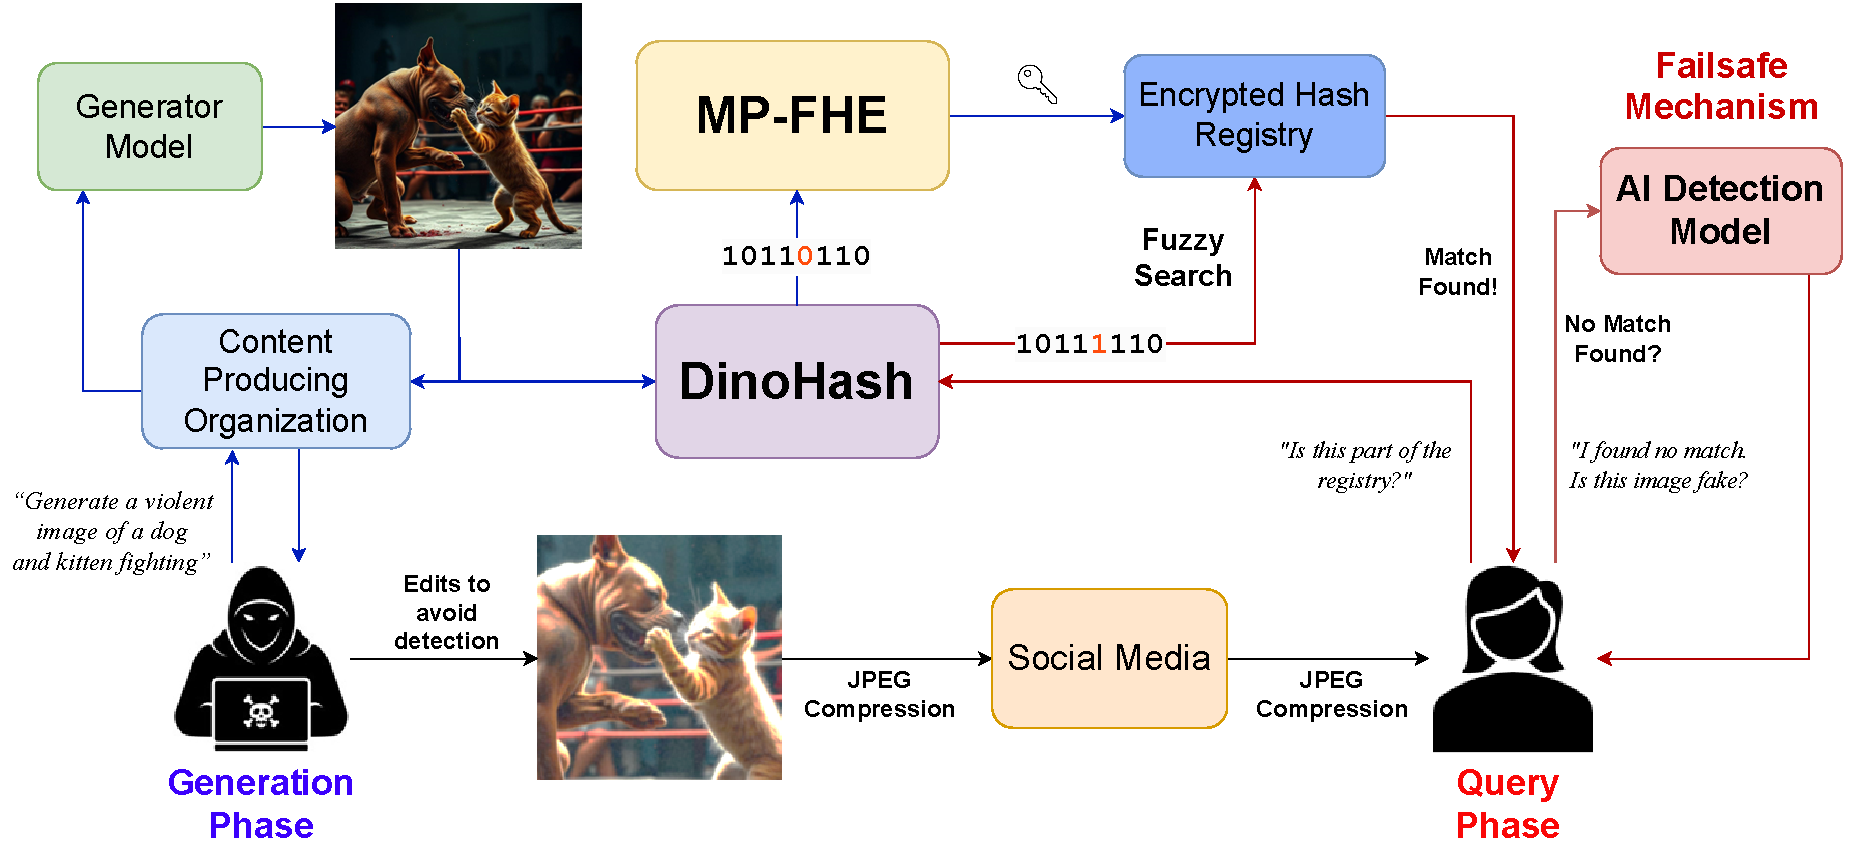
\includegraphics[width=\textwidth]{banner.pdf}
    \caption{\textbf{System Overview.} We combine the strengths of our own perceptual hashing model, DinoHash, Multi-Party Fully Homomorphic Encryption~(MP-FHE) and improved AI Detection Model to build a robust provenance framework.}
    \label{fig:teaser}
\end{figure*}

\par\noindent \textbf{Problem Definition.}  
As AI-generated media becomes increasingly prevalent, ensuring the authenticity and provenance of digital visual content has become a critical challenge. Traditional watermarking techniques are often not robust enough to withstand common image transformations, and they pose security risks when models are distributed for local use. Existing solutions like C2PA~\cite{c2pa2023} fail in practical scenarios, as their signatures become invalid after any image transformation. While proof of transformation methods~\cite{vimz, veritas} can help preserve validation after edits, the adoption of this technology by image editors remains limited. \\

\par\noindent\textbf{State-of-the-art.} Deep watermarking algorithms embed nearly invisible hashes in images, allowing later verification via specialized networks~\cite{deep_watermark}. The goals of watermarking are robustness against image distortions and minimal alteration to the original. However, these methods fail under destructive frequency-domain transformations such as blurring, JPEG compression, and screenshots, as watermarking relies on high-frequency components vulnerable to degradation through common processes like compression during social media uploads and messaging app sharing~\cite{laghari2018assessment, anwar2021image}. 

Meta's Stable Signature~\cite{meta2023stablesig} integrates watermarking directly into diffusion models, reducing inference costs. However, this requires maintaining unique model weights for each user, which becomes impractical for large-scale deployment unless models are released to users locally, creating vulnerabilities such as model purification and collusion.

Unlike watermarking, perceptual hashes derive a hash from an image’s semantic features, remaining robust against common transformations and offering a better alternative for content provenance~\cite{phash2020}. To maintain privacy, perceptual hashes must be queried without revealing sensitive data. Systems like Worldcoin’s Iris~\cite{iris-search}, Apple's Wally~\cite{wally-search}, and Panther have addressed this challenge using techniques like secure multiparty computation (MPC) and differential privacy. While Wally employs Somewhat Homomorphic Encryption (SHE), our system leverages Multi-party Fully Homomorphic Encryption (MP-FHE)~\cite{mouchet2021multiparty, lee2023efficient}, providing stronger security guarantees by ensuring multiple parties must participate in decryption.\\

\par\noindent\textbf{Proposed Method.} In response to these challenges, we propose a three-part framework designed to provide secure and reliable content provenance detection for AI-generated media in real-world settings.
Our first contribution is a perceptual hashing algorithm based on DinoV2~\cite{oquab2023dinov2}, a feature extraction network that captures the semantic and structural features of images. This alternative to watermarking is resilient to common image transformations. However, storing a perceptual hash database introduces significant privacy risks, as it may leak statistical information about end-users. For example, leaking a perceptual hash could allow partial reconstruction of an image, potentially revealing personally identifiable information~(PII)~\cite{perceptual_hash_security_2024}. Additionally, popular image generators like DALL-E store user data for up to 30 days unless de-identified or retained for legal reasons~\cite{OpenAIHelp}, making the assumption of a central database for query comparisons infeasible.

To address these privacy concerns while still enabling the benefits of a database-like structure, we propose utilizing a Multi-Party Fully Homomorphic Encryption~(MP-FHE) protocol that ensures:

\begin{itemize}
 \item \textbf{Data Confidentiality:} No entity can access any part of an image or its related information (e.g., perceptual hash) at any time.
 \item \textbf{Query Leakage Resilience:} No query or database operation will reveal or store data, either temporarily or permanently, on any device.
\end{itemize}

\noindent
To achieve this, we employ MP-FHE~\cite{mouchet2021multiparty}, which supports operations on encrypted data, enabling secure and privacy-preserving computations. This ensures that the integrity of the provenance detection process is maintained without compromising the security of sensitive data~\cite{gentry2009fully}. Additionally, we extend prior work in AI-generated content detection by training a state-of-the-art model to identify AI-generated images that may not be present in the database.


Modern tools and open-source models have democratized access to synthetic image generation. In this reality, it is unreasonable to expect every image appearing on the internet to be hashed and stored in a registry by some content-producing organization~(CPO) like cameras or AI image APIs. So, we also build a purely deep learning-based detector to perform the binary classification task of detection of synthetic images.



% \noindent In conclusion, we have three main contributions:
% \begin{itemize}
%     \item A deep perceptual hashing algorithm that is robust to a wide range of image transformations.
%     \item A cryptographic matching system that privately looks up the provenance of a perceptual hash in a registry, without leaking any data about the registry items or the queried perceptual hash.
%     \item A deep learning based detector to detect synthetic images that are not stored in the registry.
% \end{itemize}

\pagebreak

\bibliographystyle{unsrt}
\bibliography{main}

%Note
%\section{Every word is Capitalized in any \section heading in this document.}
%\subsection{Only the first word is Capitalized in any \subsection and smaller heading in this document.}


% \section{Real World Cryptography Steering Committee Bylaws}




% \section{Organizing the RWC Symposium}

% Include verbatim Section 1 (``Organizing an IACR Workshop or Conference'') of the IACR General Chair guidelines.

% In particular, the final authority for approving a symposium proposal resides
% with the IACR Board of Directors.


% \section{Timetable}
% \label{sec:timetable}

% The following timetable shows when key tasks should be completed.  All
% times are in months from time T of the symposium. 
% This timeline is specific for RWC.

% \begin{description}

% \item[T--18] A proposal by the General Chair for dates, venue, 
%   organizing committee, and a preliminary budget should be sent 
%   to the Committee.

% \item[T--13] The proposal will be selected by the Committee and 
%   approved by the Board.

% \item[T--12] Confirm the meeting place as soon as the Board has
%   approved your proposal.  If this requires payment of a deposit, set
%   up a bank account and obtain seed money from the IACR Treasurer.

% \item[T--11] 
%   Select a local organizing committee (Section~\ref{ssec:orgcomm}).
%   Refine the budget (Section~\ref{sec:budget}) and approach
%   potential sponsors for your event (Section~\ref{sec:sponsors}).
%   For RWC sponsorship is vital, and you need to be pro-active in going
%   out, finding, and contacting sponsors. Waiting for them to come to
%   you is not the way to do it.

% \item[T--9] Coordinate with the IACR webmaster and the Committee about 
%   how to host the symposium website (see Section~\ref{sec:publ}).

% \item[T--7] Finalize the budget, set a registration fee, and send the
%   detailed budget to IACR President and Treasurer for immediate review and
%   final approval (Section~\ref{sec:budget}).  You must have an
%   approved budget before registration can be opened. To set a low
%   registration fee you should have collected, or be in the process
%   of collecting most of the sponsorship by now; and hence have a
%   good idea of the final figure.

%   Inquire into obtaining insurance for the event.

% \item[T--6] Arrange and announce the registration method.  You must use the
%   IACR's own online conference registration system, which also handles
%   credit-card payments and is integrated with the IACR membership database.
%   Since all participants of IACR conferences and symposia are entitled to
%   become members of IACR, using the IACR system ensures that attendee
%   information is recorded in the membership database automatically
%   (Section~\ref{sec:registration}).

%   The possibility for registering early at a standard fee should be
%   available for at least 2 weeks after the announcement of the final
%   program.  The deadline for early registration has typically been
%   about one month before the event; careful choice of this date
%   allows you to plan ahead.

%   Announce the symposium on the website, to the IACR
%   membership by email, and open the registration 
%   (Section~\ref{ssec:announce}).  

%   If not already done, set up a bank account. Usually if you 
%   are based at a university this can be set up within your local
%   finance system at the university.

% \item[T--2] Coordinate the schedule with the program chair
%   and the Committee.

% \item[T--1] Take care of all major things to organize, like meals, coffee
%   breaks, reception, audio-visual equipment, Internet
%   access (Section~\ref{sec:major}), but also of minor things, like
%   badges (Section~\ref{sec:minor}).

%   Be prepared to send Letters of Invitation.

% \item[T--2] Monitor registrations through the IACR web interface to 
%   intercept fraudulent registrations, manage sponsoring and
%   stipends.

%   A few weeks prior to the event, you should send an email to all the
%   registered participants with some basic information and a link to the updated
%   website (program, venue, last minute changes).

% \item[T--1] 
%   At the discretion of the general chair registration fees can be increased 
%    at this point in order to encourage people to register early and facilitate your planning.
%   Experience has shown that about 80\%--90\% of the registrations come
%   in before this deadline.

% \item[T\ \ \ ] The RWC symposium takes place; see Section~\ref{sec:conference}.

% \item[T+1] Coordinate with the IACR Membership Secretary and Treasurer
%   for final attendees list, last minute registrations, refunds, address
%   changes, etc.

% \item[T+1] Start settling any outstanding financial details.

% \item[T+5] Send the financial report and surplus funds to the Treasurer.
%   Take a well-deserved rest.
% \end{description}


% \section{Proposal}
% \label{sec:proposal}

% This section explains how to prepare a proposal for
% RWC.  Before you start making a detailed proposal, you should 
% contact the Committee. 
% You will get useful feedback on how to
% proceed and on the deadline to submit your proposal.

% \subsection{Venue}
% The choice of a location involves several factors that should be
% considered early in the process.
% \begin{description}
% \item[Accessibility:]  RWC draws participants from around
% the world, and the location should be chosen with this in mind.  In the
% event of a venue located far from an international airport or major
% train station, convenient and frequent shuttle transportation should be
% made available.  Other important questions are whether IACR members
% from all countries can attend and whether you anticipate problems with visa.

% \item[Meeting facility:] The location for lectures should be large
%   enough to comfortably accommodate the expected number of
%   participants. RWC has usually had around 500 participants.
%   It is a clear
%   policy of IACR that everybody who wants to come should be allowed
%   to.  On the other hand, a meeting room that is too large will limit
%   the effectiveness of presentations and inhibit interaction.  The
%   room (or rooms) used for presentations should have at least one
%   large raised screen.  Space for
%   coffee breaks and lunches should be available nearby.  Generally
%   meeting rooms at a university are more affordable than at hotels or
%   conference centers.

%   Consider any transportation problems between lodgings and meeting
%   places.

% \item[Lodging:] Point out lodging options of different types, ranging from
%   first class (hotel) to one as cheap as possible (student dormitories
%   or equivalent).
%   Ideally,
%   participants should be able to get from lodging to the lectures and
%   back on their own and without much delay, i.e., on foot or at least
%   by public transport that runs frequently. In the latter case, make
%   precise information (also on how to get tickets) available in the
%   map or in the individual hotels.

% \item[Cost:] Many potential attendees at RWC have severely limited
%   budgets for travel.  If the cost of attending the conference is too
%   high, then many people will be unable to attend and the scientific
%   program will suffer as a result. RWC aims to keep registration low
%   by having a very high level of sponsorship. Note, that often
%   it is participants from companies and not academia which have
%   more restricted budgets; especially start-ups which are a key
%   part of the RWC target audience.
% \end{description}

% For the proposal, investigate costs of lodging, meals,
% meeting rooms, and local transportation.  It is strongly advised that
% you visit the proposed venue.  Also make sure that facilities and
% lodging will be available at the time desired.  Do all of this well in
% advance and include a set of brochures, photos, fact sheets, 
% etc.\ together with your proposal.

% \subsection{Timing}

% RWC is always in January.

% \subsection{Organizing committee}
% \label{ssec:orgcomm}

% Include verbatim Section 3.3 of the IACR General Chair guidelines.

% \subsection{Format of the proposal}

% Include verbatim Section 3.4 of the IACR General Chair guidelines.
% In particular, use the IACR \emph{conference budget planner}.

% \section{Budget}
% \label{sec:budget}

% Include verbatim Section 4 of the IACR General Chair guidelines.

% For RWC the budget for student stipends is usually between
% 20,000 and 40,000 US dollars. This is used to fund hotel
% and travel for students who would otherwise not be able to
% attend the event. Priority for this funding goes to students
% from institutions who have less access to research funds.

% \section{Sponsors}
% \label{sec:sponsors}

% Sponsoring is {\em the} major source of income for RWC.  
% Sponsors like to get recognition by having their name attached with 
% an item or to a recognizable part of the program.
% However, providing an explicit service such as this for sponsorship can
% count as a ``sales'' event; and hence can attract VAT in some
% countries. 
% Sponsorship for RWC is usually treated as a donation to the
% running of the event; mainly to support student stipends to attend
% the event.
% Sponsors should be acknowledged at the event and on the website.

% The Committee maintains strong links with sponsors for RWC.
% To this end the Committee appoints a sponsorship secretary.
% This secretary is responsible for coordinating requests for sponsorship
% to the sponsors for previous years.
% The General Chair is still responsible for finding additional sponsors to
% reduce the overall costs for attendees. The General Chair and
% the sponsorship secretary should work closely together in this respect.


% \section{Publicity}
% \label{sec:publ}

% IACR maintains a website at \url{http://www.iacr.org/}. You can
% send announcements by email to all IACR members, but you should limit
% the number of email announcements sent to all members to two for each
% event.

% The primary way for communicating with attendees is online, through
% the IACR website, the online IACR News system, the RWC website,
% and other channels (e.g., social media).  The first step is to
% list the event in the IACR calendar of events (members like to know
% dates well in advance).  To do this, fill out a
% web form at \url{http://www.iacr.org/events/}.

% The RWC website is hosted on the IACR server
% following a standard template. The Committee will be 
% responsible for sorting out the website.

% Once your basic website is set up, make sure that it is linked from the
% calendar of events and publicize the Call for Contributed Talks.
% Coordinate with the IACR Webmaster and Communications Secretary
% to announce the symposium broadly and at the appropriate time.  

% All communication regarding RWC  should clearly state that the meeting is sponsored by IACR by
% including the phrase ``sponsored by the International Association for
% Cryptologic Research.''  In addition, you should include the IACR logo
% (available from the IACR website).  If other organizations are helping
% with the meeting in some way, then you should include the phrases
% ``hosted by'' or ``in cooperation with'' for these organizations, but
% not ``sponsored by.''

% \subsection{Call for participation and other announcements}
% \label{ssec:announce}

% Include verbatim Section 6.2 of the IACR General Chair guidelines.


% \section{Registration}
% \label{sec:registration}

% Include verbatim Section 7 of the IACR General Chair guidelines.

% RWC does not foresee single-day attendance rates nor lower
% registration fees for people with lesser financial means. The
% reason being that RWC registration fees are generally quite low.
% For the same reason RWC has traditionally not allowed refunds apart from
% exceptional circumstances.  The student rate should be half the standard rate.

% \subsection{Stipends}
% \label{ssec:stipends}

% As mentioned above RWC usually has a generous student 
% stipend pot which is funded by the sponsors. 
% This should be used to waive registration fees and to 
% support lodging and transportation costs for students.

% It is recommended that the General Chair process these
% payments through the local organizing host organization.
% For example if your ``bank account'' is a university,
% then usually a university has a system for processing
% expense claims for visitors. This should be used to
% process the payment of student stipends. The reason
% for this is that different countries have different
% rules for accounting and tax status of expense
% claims. In addition, paying stipends directly from the
% IACR accounts is very complex; and thus this needs to
% be processed locally.


% \subsection{Integration into IACR membership}

% Include verbatim Section 7.7 of the IACR General Chair guidelines.


% \subsection{Registration confirmation}
% \label{ssec:confirmation}

% Include verbatim Section 7.8 of the IACR General Chair guidelines.

% \section{Major Things to Plan}
% \label{sec:major}

% Include verbatim Section 8 of the IACR General Chair guidelines,
% with the exclusion of Section~8.5 (proceedings) and 8.6 (excursion).

% Note that RWC does not normally provide any evening meals
% nor rump session, and that lunches are usually ``light'' sandwich-based
%  lunches. This is to keep registration costs down. 
% Sometimes a small drinks reception on the first day (or on
% the evening before) is organized.

% \section{Minor things to plan}
% \label{sec:minor}

% Include verbatim Section 9 of the IACR General Chair guidelines.
% Exceptions: RWC does not usually have a souvenir nor a photo to reduce
% cost; the list of attendees is available online to registered participants.

% \section{At the event}
% \label{sec:conference}

% Include verbatim Section 10 of the IACR General Chair guidelines,

% \section{Financial guidelines}
% \label{sec:financial}

% Include verbatim Section 12 of the IACR General Chair guidelines.


% \section{Preparing the program}
% \label{sec:PCGuidelines}
% This section is aimed at the Committee and the program committee for 
% a given year.

% The RWC symposium lasts for three days and consists of talks;
% about half of which are invited and half of which are contributed.
% About half the talks should be from industry and about half from
% the ``applied'' side of academia. The primary selection criteria
% are that the talks should be of interest to the audience, and that
% the speaker should be able to give a good exposition of their
% material.

% The invited talks are invited by the RWC Steering Committee, and
% are usually either about interesting topics which have occurred during
% the year, or from people in industry who the committee think
% have something interesting to say.

% Contributed talks are ``light-touch'' reviewed by a separate program committee 
% consisting of six invited reviewers, plus six members of the RWC Steering Committee. 
% The chair of the program committee is appointed by the RWC Steering Committee. 
% Usually potential contributed talks are solicited via a ``Call for Contributions''
% (the IACR {\em websubrev} system could be used for this). The ``paper'' being
% a short outline (1-2 pages) of what the talk will be about.
% The role of the program committee is to select the best such
% proposals, bearing in mind the need to maintain a balanced 
% and interesting program.

% Strong academic research results have other venues (IACR General Conferences and
% Area Conferences) and 
% product descriptions also have other venues (RSA Conference etc).
% Thus talks are selected primarily on the basis of whether the speaker
% is going to give a good talk on something which the audience will
% find interesting.

% One can sensibly fit in around six hours of talks per full day,
% assuming lengthy coffee and lunch breaks to facilitate discussions.
% Thus one expects at most 36 half hour talks over three days. Hence, 
% the goal is to obtain {\em at most} 18 contributed talks and {\em at most} 18
% invited talks. Some talks will be given a little longer than
% half an hour if the committee feel it is needed.

% \section{Levchin Prize}
% Two Levchin prizes are awarded each year. These are prizes in the
% area of real-world cryptography, which have been kindly supported by
% Max Levchin. 
% Who receives these awards is at the sole discretion of the 
% RWC Steering Committee.


% \section{More information}
% \label{app:contacts}

% More information is available on the IACR website at
% \url{http://www.iacr.org/}; browse the website and obtain information
% about past conferences and workshops.  Do not hesitate to contact 
% the members of the Committee and the Board for more information.

% The current Committee is listed on the RWC website at
% \url{https://rwc.iacr.org/}.

% The current Board is listed on the IACR website at
% \url{http://www.iacr.org/bod.html}. 


\end{document}